\documentclass{article}
\usepackage[utf8]{inputenc}
\usepackage[T1]{fontenc}

\usepackage{geometry}
\geometry{b5paper}
\usepackage{CJKutf8}

\usepackage{graphicx}
\usepackage{epstopdf}
\usepackage{multirow}
\usepackage{multicol}

\usepackage{listings}

\usepackage{pstricks}
\usepackage{pst-plot}
\usepackage{pst-func}



\usepackage{amsmath,amssymb,amsfonts} % Typical maths resource packages
\usepackage{graphics}                 % Packages to allow inclusion of graphics
%\usepackage{color}                    % For creating coloured text and background
\usepackage{xcolor}                    % For creating coloured text and background
\usepackage{hyperref}                 % For creating hyperlinks in cross references

\parindent 1cm
\parskip 0.2cm
\topmargin 0.1cm
\oddsidemargin 1cm
\evensidemargin -0.5cm
\textwidth 17cm
\textheight 23cm

\newtheorem{theorem}{Theorem}[section]
\newtheorem{proposition}[theorem]{Proposition}
\newtheorem{corollary}[theorem]{Corollary}
\newtheorem{lemma}[theorem]{Lemma}
\newtheorem{remark}[theorem]{Remark}
\newtheorem{definition}[theorem]{Definition}


\title{C++虚函数表分析\&对象的内在布局}
\author{Heyan Huang}

\usepackage{geometry}
\geometry{left=0cm,right=0cm,top=0.1cm,bottom=0cm}

\newenvironment{narrow}[2]{% 
\begin{list}{}{% 
\setlength{\topsep}{0pt}% 
\setlength{\leftmargin}{#1}% 
\setlength{\rightmargin}{#2}% 
%\setlength{\listparindent}{\parindent}% 
%\setlength{\itemindent}{\parindent}% 
\setlength{\parsep}{\parskip}% 
}% 
\item[]}{\end{list}} 
%\begin{narrow}{0.35in}{0in}  \end{narrow}


\begin{document}
\begin{CJK}{UTF8}{gbsn}
\maketitle


\small{}

\lstset{language=c++,
numbers=left, 
numberstyle=\tiny, 
%keywordstyle=\color{blue!70}, commentstyle=\color{red!55!green!55!blue!55}, 
%frame=shadowbox, 
%rulesepcolor=\color{red!20!green!20!blue!20},
escapeinside=``, 
%xleftmargin=0em,xrightmargin=0em, aboveskip=0.5em
extendedchars=false %这一条命令可以解决代码跨页时,章节标题,页眉等汉字不显示的问题
}

\section{C++虚函数表分析}

\subsection{前言}
C++中的虚函数的作用主要是实现了多态的机制。关于多态,简而言之就是用父类型别的指针指向其子类的实例,然后通过父类的指针调用实际子类的成员函数。这种技术可以让父类的指针有“多种形态”,这是一种泛型技术。所谓泛型技术,说白了就是试图使用不变的代码来实现可变的算法。比如:模板技术,RTTI技术,虚函数技术,要么是试图做到在编译时决议,要么试图做到运行时决议。
 
关于虚函数的使用方法,我在这里不做过多的阐述。大家可以看看相关的C++的书籍。在这篇文章中,我只想从虚函数的实现机制上面为大家 一个清晰的剖析。
 
当然,相同的文章在网上也出现过一些了,但我总感觉这些文章不是很容易阅读,大段大段的代码,没有图片,没有详细的说明,没有比较,没有举一反三。不利于学习和阅读,所以这是我想写下这篇文章的原因。也希望大家多给我提意见。
 
言归正传,让我们一起进入虚函数的世界。

\subsection{虚函数表}
对C++ 了解的人都应该知道虚函数(Virtual Function)是通过一张虚函数表(Virtual Table)来实现的。简称为V-Table。在这个表中,主是要一个类的虚函数的地址表,这张表解决了继承、覆盖的问题,保证其容真实反应实际的函数。这样,在有虚函数的类的实例中这个表被分配在了这个实例的内存中,所以,当我们用父类的指针来操作一个子类的时候,这张虚函数表就显得由为重要了,它就像一个地图一样,指明了实际所应该调用的函数。
 
这里我们着重看一下这张虚函数表。C++的编译器应该是保证虚函数表的指针存在于对象实例中最前面的位置(这是为了保证取到虚函数表的有最高的性能——如果有多层继承或是多重继承的情况下)。 这意味着我们通过对象实例的地址得到这张虚函数表,然后就可以遍历其中函数指针,并调用相应的函数。
 
听我扯了那么多,我可以感觉出来你现在可能比以前更加晕头转向了。 没关系,下面就是实际的例子,相信聪明的你一看就明白了。
 
假设我们有这样的一个类:
\lstinputlisting[language=c++]{vptr.cpp}
实际运行经果如下:(Windows XP+VS2003,  Linux 2.6.22 + GCC 4.1.3)
 
虚函数表地址:0012FED4

虚函数表 — 第一个函数地址:0044F148

Base::f
 
通过这个示例,我们可以看到,我们可以通过强行把\&b转成int *,取得虚函数表的地址,然后,再次取址就可以得到第一个虚函数的地址了,也就是Base::f(),这在上面的程序中得到了验证(把int* 强制转成了函数指针)。通过这个示例,我们就可以知道如果要调用Base::g()和Base::h(),其代码如下:
\begin{lstlisting}[language=c++]
            (Fun)*((int*)*(int*)(&b)+0);  // Base::f()
            (Fun)*((int*)*(int*)(&b)+1);  // Base::g()
            (Fun)*((int*)*(int*)(&b)+2);  // Base::h()
\end{lstlisting} 
这个时候你应该懂了吧。什么?还是有点晕。也是,这样的代码看着太乱了。没问题,让我画个图解释一下。如下所示:

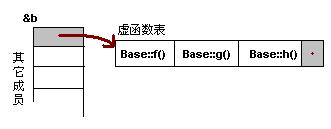
\includegraphics{m0.jpg}

注意:在上面这个图中,我在虚函数表的最后多加了一个结点,这是虚函数表的结束结点,就像字符串的结束符“/0”一样,其标志了虚函数表的结束。这个结束标志的值在不同的编译器下是不同的。在WinXP+VS2003下,这个值是NULL。而在Ubuntu 7.10 + Linux 2.6.22 + GCC 4.1.3下,这个值是如果1,表示还有下一个虚函数表,如果值是0,表示是最后一个虚函数表。
  
下面,我将分别说明“无覆盖”和“有覆盖”时的虚函数表的样子。没有覆盖父类的虚函数是毫无意义的。我之所以要讲述没有覆盖的情况,主要目的是为了给一个对比。在比较之下,我们可以更加清楚地知道其内部的具体实现。

\subsection{一般继承(无虚函数覆盖)}
下面,再让我们来看看继承时的虚函数表是什么样的。假设有如下所示的一个继承关系:

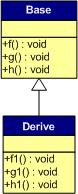
\includegraphics{m1.jpg}

请注意,在这个继承关系中,子类没有重载任何父类的函数。那么,在派生类的实例中,其虚函数表如下所示:
 
对于实例:Derive d; 的虚函数表如下:

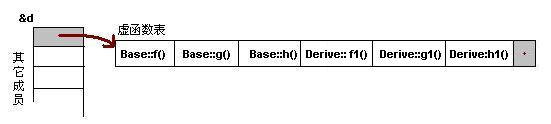
\includegraphics{m2.JPG}

我们可以看到下面几点:
\begin{enumerate}
\item 虚函数按照其声明顺序放于表中。
\item 父类的虚函数在子类的虚函数前面。
\end{enumerate}
我相信聪明的你一定可以参考前面的那个程序,来编写一段程序来验证。

\subsection{一般继承(有虚函数覆盖)}

覆盖父类的虚函数是很显然的事情,不然,虚函数就变得毫无意义。下面,我们来看一下,如果子类中有虚函数重载了父类的虚函数,会是一个什么样子?假设,我们有下面这样的一个继承关系。

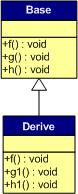
\includegraphics{m3.jpg}

为了让大家看到被继承过后的效果,在这个类的设计中,我只覆盖了父类的一个函数:f()。那么,对于派生类的实例,其虚函数表会是下面的一个样子:

 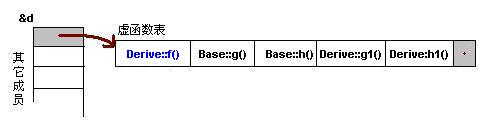
\includegraphics{m4.JPG}
 
我们从表中可以看到下面几点,
\begin{enumerate}
\item 覆盖的f()函数被放到了虚表中原来父类虚函数的位置。
\item 没有被覆盖的函数依旧。
\end{enumerate}
这样,我们就可以看到对于下面这样的程序,
\begin{lstlisting}[language=c++]
            Base *b = new Derive();
            b->f();
\end{lstlisting}
由b所指的内存中的虚函数表的f()的位置已经被Derive::f()函数地址所取代,于是在实际调用发生时,是Derive::f()被调用了。这就实现了多态。

\subsection{多重继承(无虚函数覆盖)}

 下面,再让我们来看看多重继承中的情况,假设有下面这样一个类的继承关系。注意:子类并没有覆盖父类的函数。
 
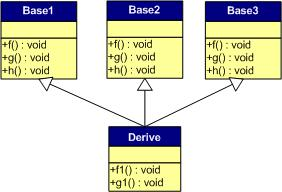
\includegraphics{m5.jpg}

对于子类实例中的虚函数表,是下面这个样子:

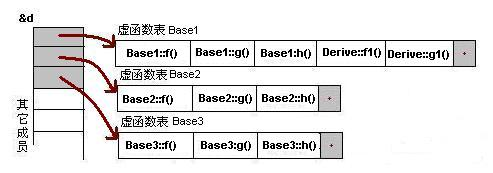
\includegraphics{m6.JPG}

 我们可以看到:
\begin{enumerate}
\item 每个父类都有自己的虚表。
\item 子类的成员函数被放到了第一个父类的表中。(所谓的第一个父类是按照声明顺序来判断的)
\end{enumerate}
这样做就是为了解决不同的父类类型的指针指向同一个子类实例,而能够调用到实际的函数。

\subsection{多重继承(有虚函数覆盖)}
下面我们再来看看,如果发生虚函数覆盖的情况。

 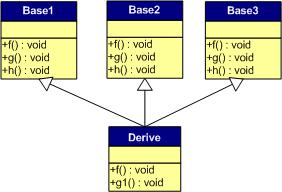
\includegraphics{m7.jpg}
 
下图中,我们在子类中覆盖了父类的f()函数。

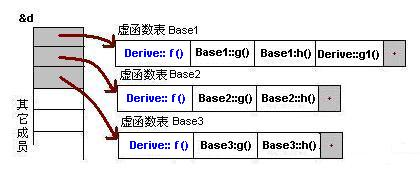
\includegraphics{m8.jpg}

我们可以看见,三个父类虚函数表中的f()的位置被替换成了子类的函数指针。这样,我们就可以任一静态类型的父类来指向子类,并调用子类的f()了。如:
\begin{lstlisting}[language=c++]
Derive d;
Base1 *b1 = &d;
Base2 *b2 = &d;
Base3 *b3 = &d;
b1->f(); //Derive::f()
b2->f(); //Derive::f()
b3->f(); //Derive::f()
 
b1->g(); //Base1::g()
b2->g(); //Base2::g()
b3->g(); //Base3::g()
\end{lstlisting} 

\subsection{安全性}
每次写C++的文章,总免不了要批判一下C++。这篇文章也不例外。通过上面的讲述,相信我们对虚函数表有一个比较细致的了解了。水可载舟,亦可覆舟。下面,让我们来看看我们可以用虚函数表来干点什么坏事吧。
\begin{description}
\item{通过父类型的指针访问子类自己的虚函数}
我们知道,子类没有重载父类的虚函数是一件毫无意义的事情。因为多态也是要基于函数重载的。虽然在上面的图中我们可以看到Base1的虚表中有Derive的虚函数,但我们根本不可能使用下面的语句来调用子类的自有虚函数:
\begin{lstlisting}[language=c++] 
          Base1 *b1 = new Derive();
            b1->f1();  //编译出错
 \end{lstlisting}
任何妄图使用父类指针想调用子类中的未覆盖父类的成员函数的行为都会被编译器视为非法,所以,这样的程序根本无法编译通过。但在运行时,我们可以通过指针的方式访问虚函数表来达到违反C++语义的行为。(关于这方面的尝试,通过阅读后面附录的代码,相信你可以做到这一点)
 
\item{访问non-public的虚函数}
另外,如果父类的虚函数是private或是protected的,但这些非public的虚函数同样会存在于虚函数表中,所以,我们同样可以使用访问虚函数表的方式来访问这些non-public的虚函数,这是很容易做到的。
\begin{lstlisting}[language=c++]
class Base {
private:
    virtual void f() { cout << "Base::f" << endl; }
};
 
class Derive : public Base{
};
 
typedef void(*Fun)(void);
void main() {
    Derive d;
    Fun  pFun = (Fun)*((int*)*(int*)(&d)+0);
    pFun();
}
\end{lstlisting}

\subsection{结束语}

C++这门语言是一门Magic的语言,对于程序员来说,我们似乎永远摸不清楚这门语言背着我们在干了什么。需要熟悉这门语言,我们就必需要了解C++里面的那些东西,需要去了解C++中那些危险的东西。不然,这是一种搬起石头砸自己脚的编程语言。
 
在文章束之前还是介绍一下自己吧。我从事软件研发有十个年头了,目前是软件开发技术主管,技术方面,主攻Unix/C/C++,比较喜欢网络上的技术,比如分布式计算,网格计算,P2P,Ajax等一切和互联网相关的东西。管理方面比较擅长于团队建设,技术趋势分析,项目管理。欢迎大家和我交流,我的MSN和Email是:haoel@hotmail.com 

\subsection{附录一:VC中查看虚函数表}

我们可以在VC的IDE环境中的Debug状态下展开类的实例就可以看到虚函数表了(并不是很完整的)

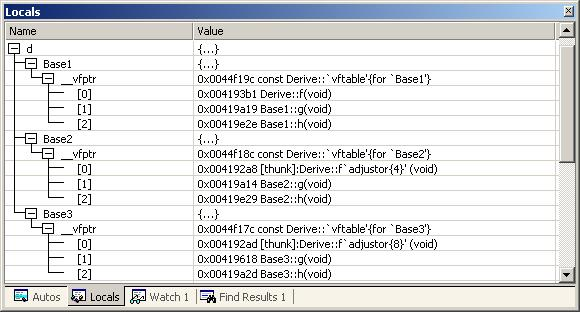
\includegraphics{m9.JPG}

\subsection{附录 二:例程}

下面是一个关于多重继承的虚函数表访问的例程:
\begin{lstlisting}[language=c++] 
#include <iostream>

using namespace std;
 
class Base1 {
public:
    virtual void f() { cout << "Base1::f" << endl; }
    virtual void g() { cout << "Base1::g" << endl; }
    virtual void h() { cout << "Base1::h" << endl; }
};
 
class Base2 {
public:
    virtual void f() { cout << "Base2::f" << endl; }
    virtual void g() { cout << "Base2::g" << endl; }
    virtual void h() { cout << "Base2::h" << endl; }
};
 
class Base3 {
public:
    virtual void f() { cout << "Base3::f" << endl; }
    virtual void g() { cout << "Base3::g" << endl; }
    virtual void h() { cout << "Base3::h" << endl; }
};
 
class Derive : public Base1, public Base2, public Base3 {
public:
    virtual void f() { cout << "Derive::f" << endl; }
    virtual void g1() { cout << "Derive::g1" << endl; }
};
 
typedef void(*Fun)(void);
 
int main()
{
    Fun pFun = NULL;
 
    Derive d;
    int** pVtab = (int**)&d;
 
    //Base1's vtable
    //pFun = (Fun)*((int*)*(int*)((int*)&d+0)+0);
    pFun = (Fun)pVtab[0][0];
    pFun();
 
    //pFun = (Fun)*((int*)*(int*)((int*)&d+0)+1);
    pFun = (Fun)pVtab[0][1];
    pFun();
 
    //pFun = (Fun)*((int*)*(int*)((int*)&d+0)+2);
    pFun = (Fun)pVtab[0][2];
    pFun();
 
    //Derive's vtable
    //pFun = (Fun)*((int*)*(int*)((int*)&d+0)+3);
    pFun = (Fun)pVtab[0][3];
    pFun();
 
    //The tail of the vtable
    pFun = (Fun)pVtab[0][4];
    cout<<pFun<<endl;
 
 
    //Base2's vtable
    //pFun = (Fun)*((int*)*(int*)((int*)&d+1)+0);
    pFun = (Fun)pVtab[1][0];
    pFun();
 
    //pFun = (Fun)*((int*)*(int*)((int*)&d+1)+1);
    pFun = (Fun)pVtab[1][1];
    pFun();
 
    pFun = (Fun)pVtab[1][2];
    pFun();
 
    //The tail of the vtable
    pFun = (Fun)pVtab[1][3];
    cout<<pFun<<endl;
 
 
    //Base3's vtable
    //pFun = (Fun)*((int*)*(int*)((int*)&d+1)+0);
    pFun = (Fun)pVtab[2][0];
    pFun();
 
    //pFun = (Fun)*((int*)*(int*)((int*)&d+1)+1);
    pFun = (Fun)pVtab[2][1];
    pFun();
 
    pFun = (Fun)pVtab[2][2];
    pFun();
 
    //The tail of the vtable
    pFun = (Fun)pVtab[2][3];
    cout<<pFun<<endl;
 
    return 0;
}
\end{lstlisting}
\end{description} 


\newpage
\section{c++对象的内存布局(上)}

\subsection{前言}

07年12月,我写了一篇《C++虚函数表解析》的文章,引起了大家的兴趣。有很多朋友对我的文章留了言,有鼓励我的,有批评我的,还有很多问问题的。我在这里一并对大家的留言表示感谢。这也是我为什么再写一篇续言的原因。因为,在上一篇文章中,我用了的示例都是非常简单的,主要是为了说明一些机理上的问题,也是为了图一些表达上方便和简单。不想,这篇文章成为了打开C++对象模型内存布局的一个引子,引发了大家对C++对象的更深层次的讨论。当然,我之前的文章还有很多方面没有涉及,从我个人感觉下来,在谈论虚函数表里,至少有以下这些内容没有涉及:
\begin{enumerate}
\item 有成员变量的情况。
\item 有重复继承的情况。
\item 有虚拟继承的情况。
\item 有钻石型虚拟继承的情况。
\end{enumerate}
这些都是我本篇文章需要向大家说明的东西。所以,这篇文章将会是《C++虚函数表解析》的一个续篇,也是一篇高级进阶的文章。我希望大家在读这篇文章之前对C++有一定的基础和了解,并能先读我的上一篇文章。因为这篇文章的深度可能会比较深,而且会比较杂乱,我希望你在读本篇文章时不会有大脑思维紊乱导致大脑死机的情况。;-)

\subsection{对象的影响因素}

简而言之,我们一个类可能会有如下的影响因素:

\begin{enumerate}
\item 成员变量
\item 虚函数(产生虚函数表)
\item 单一继承(只继承于一个类)
\item 多重继承--继承多个类
\item 重复继承--继承的多个父类中其父类有相同的超类
\item 虚拟继承(使用virtual方式继承,为了保证继承后父类的内存布局只会存在一份)
\end{enumerate} 

上述的东西通常是C++这门语言在语义方面对对象内部的影响因素,当然,还会有编译器的影响(比如优化),还有字节对齐的影响。在这里我们都不讨论,我们只讨论C++语言上的影响。
 
本篇文章着重讨论下述几个情况下的C++对象的内存布局情况。

\begin{enumerate}
\item 单一的一般继承(带成员变量、虚函数、虚函数覆盖)
\item 单一的虚拟继承(带成员变量、虚函数、虚函数覆盖)
\item 多重继承(带成员变量、虚函数、虚函数覆盖)
\item 重复多重继承(带成员变量、虚函数、虚函数覆盖)
\item 钻石型的虚拟多重继承(带成员变量、虚函数、虚函数覆盖)
\end{enumerate} 
我们的目标就是,让事情越来越复杂。

\subsection{知识复习}

我们简单地复习一下,我们可以通过对象的地址来取得虚函数表的地址,如:

\begin{lstlisting}[language=C++]
typedef void(*Fun)(void);

Base b;
Fun pFun = NULL;
 
cout << "virtual table: " << (int*)(&b) << endl;
cout << "1st function from virtual table: " << (int*)*(int*)(&b) << endl;
 
// Invoke the first virtual function 
pFun = (Fun)*((int*)*(int*)(&b));
pFun();
\end{lstlisting}
我们同样可以用这种方式来取得整个对象实例的内存布局。因为这些东西在内存中都是连续分布的,我们只需要使用适当的地址偏移量,我们就可以获得整个内存对象的布局。
 
本篇文章中的例程或内存布局主要使用如下编译器和系统:
\begin{enumerate}
\item Windows XP 和 VC++ 2003
\item Cygwin 和 G++ 3.4.4
\end{enumerate}


\subsection{单一的一般继承}

下面,我们假设有如下所示的一个继承关系:

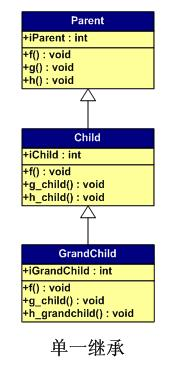
\includegraphics{mi0.jpg}

请注意,在这个继承关系中,父类,子类,孙子类都有自己的一个成员变量。而了类覆盖了父类的f()方法,孙子类覆盖了子类的g\_child()及其超类的f()。
 
我们的源程序如下所示:
\lstinputlisting[language=c++]{vptr3.cpp}
我们使用以下程序作为测试程序:(下面程序中,我使用了一个int** pVtab 来作为遍历对象内存布局的指针,这样,我就可以方便地像使用数组一样来遍历所有的成员包括其虚函数表了,在后面的程序中,我也是用这样的方法的,请不必感到奇怪,)

\begin{lstlisting}[language=c++]
  jenny@jenny-G50VT ~/docu/572/b $ g++ vptr3.cpp
  jenny@jenny-G50VT ~/docu/572/b $ ./a.out
  [0] GrandChild::_vptr->
  [0] GrandChild::f()
  [1]  Parent::g()
  [2]  Parent::h()
  [3] GrandChild::g_child()
  [4] Child::h_child()
  [5] GrandChild::h_grandchild()
  [1] Parent.iparent = 10
  [2] Child.ichild = 100
  [3] GrandChild.igrandchild = 1000
\end{lstlisting}

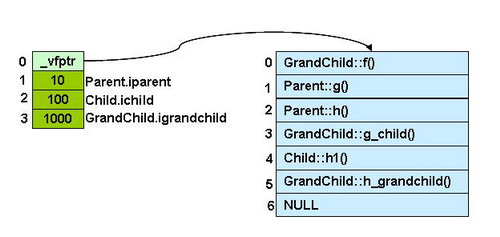
\includegraphics{mi01.jpg}

可见以下几个方面:
\begin{enumerate}
\item 虚函数表在最前面的位置。
\item 成员变量根据其继承和声明顺序依次放在后面。
\item 在单一的继承中,被overwrite的虚函数在虚函数表中得到了更新。
\end{enumerate}


\subsection{多重继承}

下面,再让我们来看看多重继承中的情况,假设有下面这样一个类的继承关系。注意:子类只overwrite了父类的f()函数,而还有一个是自己的函数(我们这样做的目的是为了用g1()作为一个标记来标明子类的虚函数表)。而且每个类中都有一个自己的成员变量:

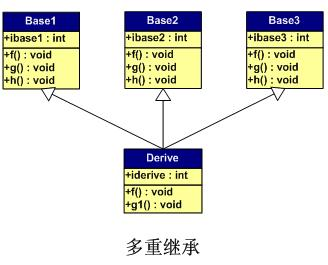
\includegraphics{mi02.jpg} 

我们的类继承的源代码如下所示:父类的成员初始为10,20,30,子类的为100
\lstinputlisting[language=c++]{vptr4.cpp}
我们通过下面的程序来查看子类实例的内存布局:下面程序中,注意我使用了一个s变量,其中用到了sizof(Base)来找下一个类的偏移量。(因为我声明的是int成员,所以是4个字节,所以没有对齐问题。关于内存的对齐问题,大家可以自行试验,我在这里就不多说了)

\begin{lstlisting}[language=c++]
jenny@jenny-G50VT ~/docu/572/b $ g++ vptr4.cpp
jenny@jenny-G50VT ~/docu/572/b $ ./a.out
[0] Base1::_vptr->
     [0] Derive::f()
     [1] Base1::g()
     [2] Base1::h()
     [3] Derive::g1()
     [4] 1
[1] Base1.ibase1 = 10
[2] Base2::_vptr->
     [0] Derive::f()
     [1] Base2::g()
     [2] Base2::h()
     [3] 1
[3] Base2.ibase2 = 20
[4] Base3::_vptr->
     [0] Derive::f()
     [1] Base3::g()
     [2] Base3::h()
     [3] 0
[5] Base3.ibase3 = 30
[6] Derive.iderive = 100
\end{lstlisting}

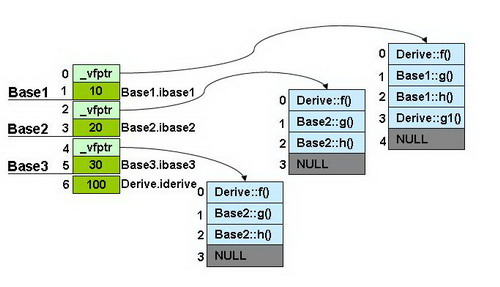
\includegraphics{mi03.jpg}

\begin{enumerate}
\item 每个父类都有自己的虚表。
\item 子类的成员函数被放到了第一个父类的表中。
\item 内存布局中,其父类布局依次按声明顺序排列。
\item 每个父类的虚表中的f()函数都被overwrite成了子类的f()。这样做就是为了解决不同的父类类型的指针指向同一个子类实例,而能够调用到实际的函数。
\end{enumerate}


\section{c++对象的内存布局(下)}

\subsection{重复继承}

下面我们再来看看,发生重复继承的情况。所谓重复继承,也就是某个基类被间接地重复继承了多次。
 
下图是一个继承图,我们重载了父类的f()函数。

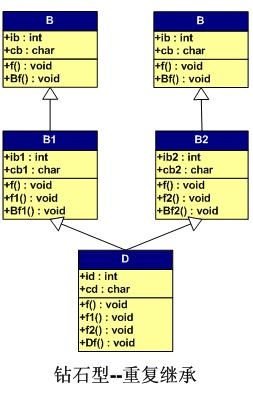
\includegraphics{mi.jpg}

其类继承的源代码如下所示。其中,每个类都有两个变量,一个是整形(4字节),一个是字符(1字节),而且还有自己的虚函数,自己overwrite父类的虚函数。如子类D中,f()覆盖了超类的函数, f1() 和f2() 覆盖了其父类的虚函数,Df()为自己的虚函数。
\lstinputlisting[language=c++]{vptr5.cpp}
程序运行结果如下:
\begin{multicols}{2}
\begin{lstlisting}[language=c++]
GCC 3.4.4 
[0] D::B1::_vptr->
     [0] D::f()
     [1] B::Bf()
     [2] D::f1()
     [3] B1::Bf1()
     [4] D::f2()
     [5] 0x1
[1] B::ib = 0
[2] B::cb = B
[3] B1::ib1 = 11
[4] B1::cb1 = 1
[5] D::B2::_vptr->
     [0] D::f()
     [1] B::Bf()
     [2] D::f2()
     [3] B2::Bf2()
     [4] 0x0
[6] B::ib = 0
[7] B::cb = B
[8] B2::ib2 = 12
[9] B2::cb2 = 2
[10] D::id = 100
[11] D::cd = D
VC++2003 
[0] D::B1::_vptr->
     [0] D::f()
     [1] B::Bf()
     [2] D::f1()
     [3] B1::Bf1()
     [4] D::Df()
     [5] 0x00000000
[1] B::ib = 0
[2] B::cb = B
[3] B1::ib1 = 11
[4] B1::cb1 = 1
[5] D::B2::_vptr->
     [0] D::f()
     [1] B::Bf()
     [2] D::f2()
     [3] B2::Bf2()
     [4] 0x00000000
[6] B::ib = 0
[7] B::cb = B
[8] B2::ib2 = 12
[9] B2::cb2 = 2
[10] D::id = 100
[11] D::cd = D
\end{lstlisting}
\end{multicols}


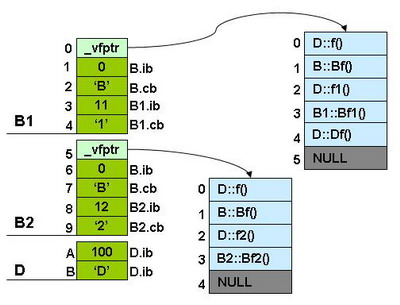
\includegraphics{dmi.jpg}

我们可以看见,最顶端的父类B其成员变量存在于B1和B2中,并被D给继承下去了。而在D中,其有B1和B2的实例,于是B的成员在D的实例中存在两份,一份是B1继承而来的,另一份是B2继承而来的。所以,如果我们使用以下语句,则会产生二义性编译错误:
\begin{lstlisting}[language=c++]
D d;
d.ib = 0;               //two meaning
d.B1::ib = 1;           //correct
d.B2::ib = 2;           //
\end{lstlisting}
注意,上面例程中的最后两条语句存取的是两个变量。虽然我们消除了二义性的编译错误,但B类在D中还是有两个实例,这种继承造成了数据的重复,我们叫这种继承为重复继承。重复的基类数据成员可能并不是我们想要的。所以,C++引入了虚基类的概念。

\subsection{钻石型多重虚拟继承}
虚拟继承的出现就是为了解决重复继承中多个间接父类的问题的。钻石型的结构是其最经典的结构。也是我们在这里要讨论的结构:
 
上述的“重复继承”只需要把B1和B2继承B的语法中加上virtual关键,就成了\\
虚拟继承,其继承图如下所示:

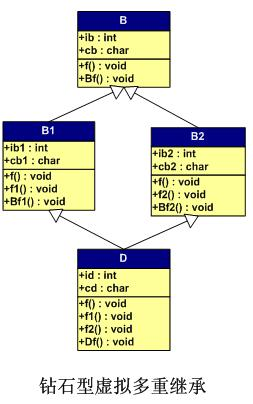
\includegraphics{mi2.jpg}

上图和前面的“重复继承”中的类的内部数据和接口都是完全一样的,只是我们采用了\\
虚拟继承:其省略后的源码如下所示:
\begin{lstlisting}[language=c++]
class B {……};
class B1 : virtual public B{……};
class B2: virtual public B{……};
class D : public B1, public B2{ …… };
\end{lstlisting} 
 
在查看D之前,我们先看一看单一虚拟继承的情况。下面是一段在VC++2003下的测试程序:(因为VC++和GCC的内存而局上有一些细节上的不同,所以这里只给出VC++的程序,GCC下的程序大家可以根据我给出的程序自己仿照着写一个去试一试):
\begin{lstlisting}[language=c++]
int** pVtab = NULL;
    Fun pFun = NULL;
    B1 bb1;
 
    pVtab = (int**)&bb1;
    cout << "[0] B1::_vptr->" << endl;
    pFun = (Fun)pVtab[0][0];
    cout << "     [0] ";
    pFun(); //B1::f1();
    cout << "     [1] ";
    pFun = (Fun)pVtab[0][1];
    pFun(); //B1::bf1();
    cout << "     [2] ";
    cout << pVtab[0][2] << endl;
 
    cout << "[1] = 0x";
    cout << (int*)*((int*)(&bb1)+1) <<endl; //B1::ib1
    cout << "[2] B1::ib1 = ";
    cout << (int)*((int*)(&bb1)+2) <<endl; //B1::ib1
    cout << "[3] B1::cb1 = ";
    cout << (char)*((int*)(&bb1)+3) << endl; //B1::cb1
 
    cout << "[4] = 0x";
    cout << (int*)*((int*)(&bb1)+4) << endl; //NULL
 
    cout << "[5] B::_vptr->" << endl;
    pFun = (Fun)pVtab[5][0];
    cout << "     [0] ";
    pFun(); //B1::f();
    pFun = (Fun)pVtab[5][1];
    cout << "     [1] ";
    pFun(); //B::Bf();
    cout << "     [2] ";
    cout << "0x" << (Fun)pVtab[5][2] << endl;
 
    cout << "[6] B::ib = ";
    cout << (int)*((int*)(&bb1)+6) <<endl; //B::ib
    cout << "[7] B::cb = ";
\end{lstlisting}

其运行结果如下(我结出了GCC的和VC++2003的对比):

\begin{multicols}{2}
\begin{lstlisting}[language=c++]
GCC 3.4.4
[0] B1::_vptr ->
    [0] : B1::f()
    [1] : B1::f1()
    [2] : B1::Bf1()
    [3] : 0
[1] B1::ib1 : 11
[2] B1::cb1 : 1
[3] B::_vptr ->
    [0] : B1::f()
    [1] : B::Bf()
    [2] : 0
[4] B::ib : 0
[5] B::cb : B
[6] NULL : 0
VC++ 2003
[0] B1::_vptr->
     [0] B1::f1()
     [1] B1::Bf1()
     [2] 0
[1] = 0x00454310 ç该地址取值后是-4
[2] B1::ib1 = 11
[3] B1::cb1 = 1
[4] = 0x00000000
[5] B::_vptr->
     [0] B1::f()
     [1] B::Bf()
     [2] 0x00000000
[6] B::ib = 0
[7] B::cb = B
\end{lstlisting}
\end{multicols}

这里,大家可以自己对比一下。关于细节上,我会在后面一并再说。
 
下面的测试程序是看子类D的内存布局,同样是VC++ 2003的(因为VC++和GCC的内存布局上有一些细节上的不同,而VC++的相对要清楚很多,所以这里只给出VC++的程序,GCC下的程序大家可以根据我给出的程序自己仿照着写一个去试一试):
\begin{lstlisting}[language=c++]
    D d;
 
    pVtab = (int**)&d;
    cout << "[0] D::B1::_vptr->" << endl;
    pFun = (Fun)pVtab[0][0];
    cout << "     [0] ";    pFun(); //D::f1();
    pFun = (Fun)pVtab[0][1];
    cout << "     [1] ";    pFun(); //B1::Bf1();
    pFun = (Fun)pVtab[0][2];
    cout << "     [2] ";    pFun(); //D::Df();
    pFun = (Fun)pVtab[0][3];
    cout << "     [3] ";
    cout << pFun << endl;
 
    //cout << pVtab[4][2] << endl;
    cout << "[1] = 0x";
    cout <<  (int*)((&dd)+1) <<endl; //????
 
    cout << "[2] B1::ib1 = ";
    cout << *((int*)(&dd)+2) <<endl; //B1::ib1
    cout << "[3] B1::cb1 = ";
    cout << (char)*((int*)(&dd)+3) << endl; //B1::cb1
 
    //---------------------
    cout << "[4] D::B2::_vptr->" << endl;
    pFun = (Fun)pVtab[4][0];
    cout << "     [0] ";    pFun(); //D::f2();
    pFun = (Fun)pVtab[4][1];
    cout << "     [1] ";    pFun(); //B2::Bf2();
    pFun = (Fun)pVtab[4][2];
    cout << "     [2] ";
    cout << pFun << endl;
   
    cout << "[5] = 0x";
    cout << *((int*)(&dd)+5) << endl; // ???
 
    cout << "[6] B2::ib2 = ";
    cout << (int)*((int*)(&dd)+6) <<endl; //B2::ib2
    cout << "[7] B2::cb2 = ";
    cout << (char)*((int*)(&dd)+7) << endl; //B2::cb2
 
    cout << "[8] D::id = ";
    cout << *((int*)(&dd)+8) << endl; //D::id
    cout << "[9] D::cd = ";
    cout << (char)*((int*)(&dd)+9) << endl;//D::cd
 
    cout << "[10]  = 0x";
    cout << (int*)*((int*)(&dd)+10) << endl;

    //---------------------
    cout << "[11] D::B::_vptr->" << endl;
    pFun = (Fun)pVtab[11][0];
    cout << "     [0] ";    pFun(); //D::f();
    pFun = (Fun)pVtab[11][1];
    cout << "     [1] ";    pFun(); //B::Bf();
    pFun = (Fun)pVtab[11][2];
    cout << "     [2] ";
    cout << pFun << endl;
 
    cout << "[12] B::ib = ";
    cout << *((int*)(&dd)+12) << endl; //B::ib
    cout << "[13] B::cb = ";
    cout << (char)*((int*)(&dd)+13) <<endl;//B::cb
\end{lstlisting}

\begin{multicols}{2}
\begin{lstlisting}[language=c++]
GCC 3.4.4
[0] B1::_vptr ->
    [0] : D::f()
    [1] : D::f1()
    [2] : B1::Bf1()
    [3] : D::f2()
    [4] : D::Df()
    [5] : 1
[1] B1::ib1 : 11
[2] B1::cb1 : 1
[3] B2::_vptr ->
    [0] : D::f()
    [1] : D::f2()
    [2] : B2::Bf2()
    [3] : 0
[4] B2::ib2 : 12
[5] B2::cb2 : 2
[6] D::id : 100
[7] D::cd : D
[8] B::_vptr ->
    [0] : D::f()
    [1] : B::Bf()
    [2] : 0
[9] B::ib : 0
[10] B::cb : B
[11] NULL : 0
VC++ 2003
[0] D::B1::_vptr->
     [0] D::f1()
     [1] B1::Bf1()
     [2] D::Df()
     [3] 00000000
[1] = 0x0013FDC4  ç 该地址取值后是-4
[2] B1::ib1 = 11
[3] B1::cb1 = 1
[4] D::B2::_vptr->
     [0] D::f2()
     [1] B2::Bf2()
     [2] 00000000
[5] = 0x4539260   ç 该地址取值后是-4
[6] B2::ib2 = 12
[7] B2::cb2 = 2
[8] D::id = 100
[9] D::cd = D
[10]  = 0x00000000
[11] D::B::_vptr->
     [0] D::f()
     [1] B::Bf()
     [2] 00000000
[12] B::ib = 0
[13] B::cb = B

\end{lstlisting}
\end{multicols}
关于虚拟继承的运行结果我就不画图了(前面的作图已经让我产生了很严重的厌倦感,所以就偷个懒了,大家见谅了)
 
在上面的输出结果中,我用不同的颜色做了一些标明。我们可以看到如下的几点:
 \begin{enumerate}
\item 无论是GCC还是VC++,除了一些细节上的不同,其大体上的对象布局是一样的。也就是说,先是B1(黄色),然后是B2(绿色),接着是D(灰色),而B这个超类(青蓝色)的实例都放在最后的位置。
\item 关于虚函数表,尤其是第一个虚表,GCC和VC++有很重大的不一样。但仔细看下来,还是VC++的虚表比较清晰和有逻辑性。
\item VC++和GCC都把B这个超类放到了最后,而VC++有一个NULL分隔符把B和B1和B2的布局分开。GCC则没有。
\item VC++中的内存布局有两个地址我有些不是很明白,在其中我用红色标出了。取其内容是-4。接道理来说,这个指针应该是指向B类实例的内存地址(这个做法就是为了保证重复的父类只有一个实例的技术)。但取值后却不是。这点我目前还并不太清楚,还向大家请教。
\item GCC的内存布局中在B1和B2中则没有指向B的指针。这点可以理解,编译器可以通过计算B1和B2的size而得出B的偏移量。
\end{enumerate}
  
\subsection{结束语}
C++这门语言是一门比较复杂的语言,对于程序员来说,我们似乎永远摸不清楚这门语言背着我们在干了什么。需要熟悉这门语言,我们就必需要了解C++里面的那些东西,需要我们去了解他后面的内存对象。这样我们才能真正的了解C++,从而能够更好的使用C++这门最难的编程语言。
 
在文章束之前还是介绍一下自己吧。我从事软件研发有十个年头了,目前是软件开发技术主管,技术方面,主攻Unix/C/C++,比较喜欢网络上的技术,比如分布式计算,网格计算,P2P,Ajax等一切和互联网相关的东西。管理方面比较擅长于团队建设,技术趋势分析,项目管理。欢迎大家和我交流,我的MSN和Email是:haoel@hotmail.com 


\section{c++中的基类与派生类}

派生类的继承方式总结:

\begin{tabular}{|l|l|}
\hline
\hline
继承方式 & 说明\\
\hline
\hline
public & 基类的public和protected的成员被派生类继承后,保持原来的状态\\
\hline
private & 基类的public和protected的成员被派生类继承后,变成派生类的private成员\\
\hline
protected & 基类的public和protected的成员被派生类继承后,变成派生类的protected成员\\
\hline
\hline
\end{tabular}

注:无论何种继承方式,基类的private成员都不能被派生类访问。从上面的表中可以看出,声明为public的方法和属性可以被随意访问;声明为protected的方法和属性只能被类本身和其子类访问;而声明为private的方法和属性只能被当前类的对象访问。 
\begin{enumerate}
\item 友元函数必须在类中进行声明而在类外定义,声明时须在函数返回类型前面加上关键字friend。友元函数虽不是类的成员函数,但它可以访问类中的私有和保护类型数据成员。  
\item 虚函数在重新定义时参数的个数和类型必须和基类中的虚函数完全匹配,这一点和函数重载完全不同。  
\item \#include <文件名>和\#include "文件名"  
\begin{itemize}
\itemsep=-3pt
\item 文件包含的两种格式中,第一种格式用来包含那些由系统提供的并放在指定子目录中的头文件;而第二种格式用来包含那些由用户自己定义的放在当前目录或其他目录下的头文件或其它源文件。  
\end{itemize}
\item 数组也可以作为函数的实参和形参,若数组元素作为函数的实参,则其用法与变量相同。当数组名作为函数的实参和形参时,传递的是数组的地址。当进行按值传递的时候,所进行的值传送是单向的,即只能从实参传向形参,而不能从形参传回实参。形参的初值和实参相同,而形参的值发生改变后,实参并不变化,两者的终值是不同的。而当用数组名作为函数参数进行传递时,由于实际上实参和形参为同一数组,因此当形参数组发生变化时,实参数组也随之发生变化。  

注:实参数组与形参数组类型应一致,如不一致,结果将出错;形参数组也可以不指定大小,在定义数组时数组名后面跟一个空的方括号,为了在被调用函数中处理数组元素的需要,可以另设一个参数,传递数组元素的个数。如:int sum(int array[],int n);  
\item 重载、覆盖和隐藏的区别?  

函数的重载是指C++允许多个同名的函数存在,但同名的各个函数的形参必须有区别:形参的个数不同,或者形参的个数相同,但参数类型有所不同。 

覆盖(Override)是指派生类中存在重新定义的函数,其函数名、参数列、返回值类型必须同父类中的相对应被覆盖的函数严格一致,覆盖函数和被覆盖函数只有函数体 (花括号中的部分)不同,当派生类对象调用子类中该同名函数时会自动调用子类中的覆盖版本,而不是父类中的被覆盖函数版本,这种机制就叫做覆盖。
\end{enumerate} 
下面我们从成员函数的角度来讲述重载和覆盖的区别。

成员函数被重载的特征有: 
\begin{enumerate}
\item 相同的范围(在同一个类中);
\item 函数名字相同;
\item 参数不同;
\item virtual关键字可有可无。
\end{enumerate}

覆盖的特征有: 
\begin{enumerate} \itemsep=-3pt
\item 不同的范围(分别位于派生类与基类);
\item 函数名字相同;
\item 参数相同;
\item 基类函数必须有virtual关键字。
\end{enumerate}

隐藏是指派生类的函数屏蔽了与其同名的基类函数,规则如下: 
\begin{itemize}
\itemsep=-3pt
\item 如果派生类的函数与基类的函数同名,但是参数不同。此时,不论有无virtual关键字,基类的函数将被隐藏(注意别与重载混淆)。
\item 如果派生类的函数与基类的函数同名,并且参数也相同,但是基类函数没有virtual关键字。此时,基类的函数被隐藏(注意别与覆盖混淆)。
\end{itemize}

重载(overload):这个好理解,在同个space域同名的。参数必须不同,有关virtual无关.

覆盖(override):同名字,同参数,有virtual,覆盖好理解比如show()函数,A派生了B,如果B中的show()覆盖了A中的show(),但B中仍然有两个show(),而不管是A类指针也好,B类对象调用也好,都只能调用B类自己的那个show();而从A类继承过来的show()函数真的就被覆盖了,没有了吗? 答案是不对的.这时可以在B类对象显示的调用A类继承过来的show();

隐藏hide:
\begin{enumerate}
\itemsep=-3pt
\item 同名同参无virtual
\item 同名不同参不管有无virtual
\end{enumerate}

\subsection{派生类与基类之间的关系}

派生类对象可以使用基类的方法,条件是方法在基类中没有被声明为私有的。基类指针可以在不进行显式类型转换的情况下指向派生类对象,基类引用可以在不进行显式类型转换的情况下引用派生类对象。不过,基类指针或引用只能用于调用基类方法,不能调用派生类的方法。通常C++要求引用和指针类型与赋给的类型匹配,但这一规则对继承来说是个例外。不过这种例外只是单向的,不可以将基类对象和地址赋给派生类引用和指针。

\subsection{静态联编和动态联编}

程序调用函数时,将使用哪个可执行代码块呢?编译器负责回答这个问题。将源代码中的函数调用解释为执行特定的函数代码块被称为函数名联编。在C语言中,这非常简单,因为每个函数名都对应一个不同的函数。在C++中,由于函数重载的缘故,这项任务更复杂。编译器必须查看函数参数以及函数名才能确定使用哪个函数。然而,C/C++编译器可以在编译过程完成这种联编。在编译过程中进行联编被称为静态联编/绑定,又称为早期联编/绑定。不过,虚函数使这项工作变得更困难。因为使用哪个函数是不能在编译时确定的,因为编译器不知道用户将选择哪种类型的对象。所以,编译器必须生成能够在程序运行时选择正确的虚方法的代码,这被称为动态联编/绑定,又被称为晚期联编/绑定。

\subsection{运算符重载}

\subsubsection{区别于函数重载,运算符重载有一下限制:}
\begin{itemize}
\itemsep=-3pt
\item 只能对C++现有运算符进行重载
\item 不能改变参加运算的操作数的个数
\item 不能改变运算符原有的优先级和结合性
\end{itemize}

\subsubsection{C++中大多数运算符都可以重载,但以下运算符不允许重载:}
\begin{itemize}
\itemsep=-3pt
\item 成员运算符 : "."
\item 作用域限定符 : "::"
\item 条件运算 : "?:"
\item 计算占用内存 : "sizeof()"
\end{itemize}

\subsection{基类指针指向派生类对象}
根据C++指针的定义,一种类型的指针不能指向另一种类型的变量。
\begin{itemize}
\itemsep=-3pt
\item 基类指针可以指向派生类的对象
\item 派生类指针不可以指向基类对象
\item 注意:即使将一个基类的指针指向一个派生类的对象,通过该指针也只能访问派生类中从基类继承来的共有成员,不能访问派生类中新增加的成员,\
\end{itemize}
除非通过强制转换将基类指针转换为派生类指针

\section{C++ NEW的使用及 基类指针转换成派生类指针 \&\\
static\_cast和dynamic\_cast的说明}

\subsection{new的使用}
\begin{enumerate}
\itemsep=-3pt
\item new() 分配这种类型的一个大小的内存空间,并以括号中的值来初始化这个变量;
\item new[] 分配这种类型的n个大小的内存空间,并用默认构造函数来初始化这些变量; 
\item 当使用new运算符定义一个多维数组变量或数组对象时,它产生一个指向数组第一个元素的指针,返回的类型保持了除最左边维数外的所有维数
\end{enumerate}

\subsection{基类指针转换成派生类指针}
\begin{lstlisting}[language=c++]
class Base;
class Child: Base
Base* Cba=new Child(); //相当于把基类Base的指针指向一个子类Chid开辟的对象,这个空间包含从Base继承
\end{lstlisting}

而来的和Child独有的成员,但是因为声明指针为Base*类型,因此只能通过这个指针存取从基类继承的成员变量和成员函数,而不能存取子类Child自己声明的东西,因为基类指针并不能知道子类都有哪些扩展~~,如果想使用

派生类的声明的,就需要把基类转换为派生类。

基类转换为派生类转换方法2种,
\begin{itemize}
\itemsep=-3pt
\item 基类强制转换成派生类(不推荐)。
\item 使用dynaminc\_cast进行转换(推荐);
\end{itemize}

Child*Cch=new Base();//这样是错误的...因为违背了(按照指针变量的定义,Base指针类型地址里面存放的应是Base类型的变量),而Base* Cba=new Child();为什么是可以的,因为任何一个(子类)Child对象同时也是一个合法的(父类)Base对象。C++允许基类的指针指向派生类的是为了方便代码的重用,比如虚函数。

\subsection{static\_cast和dynamic\_cast的区别}
\begin{itemize}
\itemsep=-3pt
\item static\_cast转换类似于C/C++里面的强制类型转换。   

   dynaminc\_cast主要用在继承树上的向下转换,转换是根据基类派生类的原则进行转换,如果无法转换,返回NULL或抛出异常.(把基类转换为派生类). (如果是dynamic\_cast<T*>(foo)失败,返回的是NULL,但是如果是dynamic\_cast<T\&>(foo)失败,结果是抛出一个bad\_cast的异常)

\item dynamic\_cast是一个运行期借助于RTTI的操作符,而static\_cast不是   
\item 只有申明了虚拟函数的类才能使用dynamic\_cast操作符。多态是通过VPTB实现的。   

C语言的结构(没有多态)才能使用static\_cast,否则将出错。
\end{itemize}


\end{CJK}
\end{document}
